\section{Architektura aplikacji}
\label{chapter:application:architecture}

\begin{figure}[H]
    \centering
    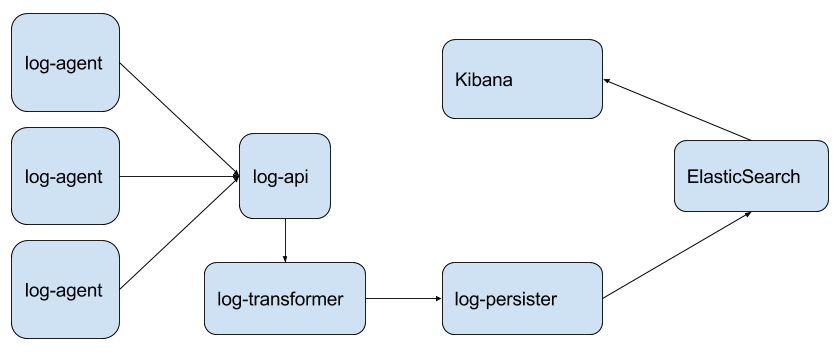
\includegraphics[width=1.0\textwidth]{images/application_arch}
    \caption[Architektura aplikacji]{
        Architektura aplikacji, źródło: opracowanie własne
    }
    \label{chapter:application:architecture:diagram}
\end{figure}

Część praktyczna pracy dyplomowej, przedstawiona na rysunku \ref{chapter:application:architecture:diagram}, 
zaprojektowana została w architekturze rozproszonej - mikro serwisu. Głównym zadaniem takiego rozwiązania
jest rozbicie faktycznej aplikacji na mniejsze programy. Poszczególne części składowe posiadają jedno, 
jasno określone, zadania i jedynie za nie są odpowiedzialne. Niemniej, zasada pojedynczej odpowiedzialności, znana także jako
jeden z wyznaczników dobrej klasy w rozumieniu programowania obiektowego, jest także i tutaj rozumiana w szerszym
kontekście. Pojedynczy serwis współpracuje z innymi. Przykładowa aplikacja mogłaby realizować funkcjonalność 
sklepu internetowego. Jednymi z wielu zamkniętych w środków serwisów, mogłyby by być te odpowiedzialne za zarządzania
klientami lub ogólnie użytkownikami oraz te, których zadaniem byłoby, wsparcie w kierunku zarządzania towarami oferowanymi
przez sklep. Oba, z kolei, wymagałyby wsparcia kolejnego serwisu - bazy danych. Z przedstawionego opisu wynikają jasno pewne
szczególne cechy tego typu architektury:
\begin{itemize}
    \item[\textbf{skalowalność}] - konieczność uruchomienia kolejnych serwisów tego samego typu nie jest trudnym zadaniem. Dzięki temu, 
    że są to aplikacje małe, są one jednocześnie łatwe w zarządzaniu. Ponadto skalowania w kierunku osi OY jest tańsze. Koszt
    dodania średniej mocy maszyny, na której działałaby kolejne instancja serwisu, jest niższy niż dołożenia szybszych podzespołów
    do już istniejącej maszyny, co jest cechą znamienną skalowania wertykalnego,
    \item[\textbf{nauczenie się aplikacji}] - łatwiej jest zrozumieć prostą aplikację, mechanizmy jej działania, aniżeli dogłębnie poznać
    jedną większą. Okazuje się to szczególnie przydatne w dynamicznych zespołach programistów, gdzie rotacja ludzi jest wysoka albo
    częstym zmianą podlegają wymagania,
    \item[\textbf{lepsze izolowanie}] - żaden program nie jest wolny od błędów. Izolowania poszczególnych serwisów jest szczególnie
    przydatne, jeśli dana aplikacja ma problemy z zarządzaniem pamięcią lub przestrzenią dyskową. Inwestygacja mająca 
    na celu ustalenie problemu w dużym programie zajęłaby dużo więcej czasu, nie wspominając już o jego wyeliminowania. 
    W małych aplikacjach ilość wzajemnych korelacji między poszczególnymi jej komponentami jest znacznie niższa od tej
    spotykanych w średnich i dużych programach,
    \item[\textbf{niezależność}] - model aktualizacji lub bardziej ogólnie przekazywania gotowej aplikacji do środowiska produkcyjnego
    staje się również uproszczony. W architekturze mikro-serwisów, każdy serwis może być rozwijany niezależnie od innych i 
    w takiej samej formie, można wypuszczać jego nowe wersje. Jest to także udogodnienie dla klientów, którzy mogą
    pobrać jedynie mały plik binarny lub archiwum. Sam proces aktualizacji jest również narażony na mniejszą ilość
    trudnych do przewidzenia problemu \cite{microservice_architecture}. 
\end{itemize}

Najważniejszą jednak cechą, z którą borykają się systemy informatyczne, jest wyeliminowania \textbf{single-point-of-failure}.
To angielskie pojęcia, w praktyce oznaczana, wadę architektury systemu lub nawet i aplikacji. Najczęściej jednak odnosi się
ona do systemu jako całości. Umieszczenie w jednym miejscu jednej dużej aplikacji lub kilku mniejszych współpracujących 
między sobą, powoduje powstania newralgicznego punktu całego systemu, który jeśli ulegnie awarii, w najlepszy wypadku spowoduje
jedynie opóźnienie w dostarczaniu potrzebnych usług, a w najgorszym całkowicie wyłączy system. Warto w tym miejscu dodać, że
awarie, nie muszą być wcale spowodowane przez sam program. Sytuacje takie jak wyczerpania się pamięci operacyjnej lub 
zajęcia całej mocy obliczeniowej procesora, stanowią ułamek możliwych niefortunnych komplikacji. Należy tutaj brać pod uwagę
także awarię sprzętu, przerwy w dostawie prądu, a także konieczność przeprowadzania prac serwisów lub wymiany istniejących
komponentów komputera na lepsza.  

\subsection{Proces instalacji}
\label{chapter:application:architecture:installation}
    Część praktyczna, jak zostało wcześniej omówione, została zrealizowana w architekturze mikro-serwisów. Warto w tym miejscu dodać,
    że oprócz komponentów omówionych w poniższych rozdziałach, jest to tak naprawdę rozszerzenie istniejącego rozwiązania typu \textbf{MaaS}
    (\ref{chapter:monitoring_architecture:maas}) - monasca. W przypadku tak dużego systemu, składającego się z wielu elementów, 
    konieczne było opracowanie spójnej metody instalacji. Wybór padł na \textbf{Ansible}. 
    
    \subsubsection{Ansible - Simple IT Automation}
    \label{chapter:application:architecture:installation:ansible}
    Ansible jest odpowiedzią na pytania - Jak wdrożyć kompleksowy system na więcej niż jednej maszynie. Architektura tego rozwiązania,
    zakłada przygotowanie pakietów instalacyjnych w relacji 1:1 do komponentu, który ma on instalować. Wspomniany pakiet, istnieje pod nazwą roli.
    Jest to najmniejsza cegiełka w całym ekosystemie. Domem, korzystając w dalszej części z metafory, jest tak zwany \textbf{playbook}.
    
    \begin{figure}[h]
        \centering
        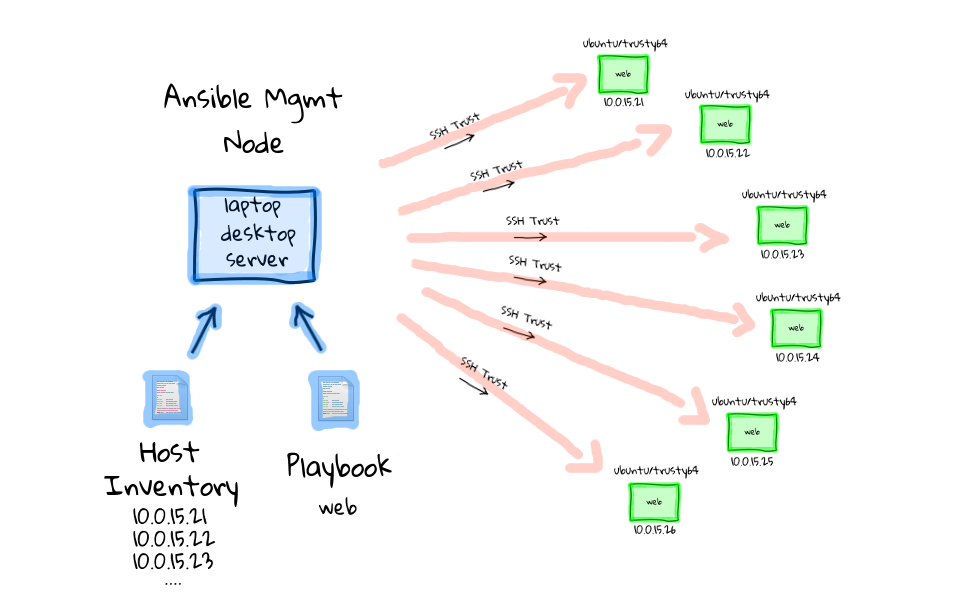
\includegraphics[width=1.0\textwidth]{images/43-ansible-multi-node-deployment-workflow}
        \caption[Wdrożenia z Ansible]{
            Wdrożenia z Ansible, 
            źródło: \url{https://d1cg27r99kkbpq.cloudfront.net/static/extra/43-ansible-multi-node-deployment-workflow.png}
        }
        \label{chapter:application:architecture:installation:ansible_diagram}
    \end{figure}
     
    Pozwala on na budowania scenariusza instalacji według koncepcji przedstawionej na diagramie 
    \ref{chapter:application:architecture:installation:ansible_diagram}. Pojedyncza maszyna, zwana dalej
    maszyną kontrolną, posiada wiedzę o wszystkich hostach wchodzących w skład całego systemu. Na niej
    również zlokalizowane są scenariusze. Ręcznie lub automatyczne zarządzenie infrastrukturą jest
    tutaj aspektem wykraczającym poza ramy pracy dyplomowej, dlatego też nie zostanie omówione. 
    Warto jedynie dodać, że sam proces instalacji na maszynach, możliwy jest do monitorowania na co najmniej
    dwa sposoby:
    
    \begin{itemize}
        \item[Ansible Tower] - rozwiązanie zaprojektowane specjalnie z myślą o monitorowaniu pracy
        procesu wdrożeniowego. Pozwala na przeglądanie listy wszystkich maszyn, obecnego statusu
        zadań (ról),
        \item[Syslog] - wszelka aktywność (tj. operacja), które \textbf{Ansible} wykonuje logowane są
        z użyciem protokołu Syslog na danej maszynie. Dostęp do logów pozwala na prześledzenie operacji oraz
        ewentualnego uzyskania wiedzy na temat przyczyn nieprawidłowego (zakończonego niepowodzeniem) wdrożenia
    \end{itemize}
    
    Najistotniejszą cechą \textbf{Ansible} jest jednak możliwość wskazania, praktycznie nieskończonej,
    ilości maszyn docelowych (fizycznych, wirtualnych lub nawet kontenerów Docker), na których ma zostać ona wprowadzona. 
    Dzięki temu, skalowanie aplikacji na kolejne maszyny, przestaje być operacją problematyczną. Wystarczy dodać 
    informację o jej adresie IP oraz skonfigurować komunikację protokołem SSH.
